\documentclass[12pt, conference, a4paper]{article}
\usepackage{a4wide}
\usepackage[centertags]{amsmath}
\usepackage{amsfonts,amssymb,amsthm}
\usepackage{graphicx}
\usepackage{wrapfig}
\usepackage{iitbcstitle}
% \usepackage{listings}
% \usepackage{xcolor}
% \usepackage{xparse}
\usepackage[]{minted}
\usepackage{biblatex} 
\usepackage{url}
\usepackage{hyperref}
\usepackage{todonotes}
\usepackage[none]{hyphenat}
\usepackage{enumitem}
\usepackage{booktabs}
\usepackage{float}
\linespread{1.15}
\usepackage[cm]{fullpage}
\usepackage{rotating}
\usepackage{times}
\usepackage{textcomp}
\usepackage{caption}
\usepackage{subcaption}
\setlength\parindent{0pt}
\addbibresource{references.bib}

\begin{document}

\title{\Huge APRICOT and SAFE \\ \large RnD report and Documentation
}
\author{
  \small
\begin{tabular}{c}  {Bhaveshkumar Yadav} \\ bhaveshy@iitb.ac.in \\ Guide: Prof. Bhaskaran Raman \\ \footnotesize Department of Computer Science \& Engineering \\ IIT Bombay \end{tabular} }

\maketitle
\pagenumbering{arabic}



\section{Introduction}
\label{SEC:introduction}
This report is the documentation of the work done on the SAFE and APRICOT app for iOS during the spring semester of 2019-20. SAFE (Smart, Authenticated, Fast Exams) is an application system used in IIT Bombay and 30+ other colleges for conducting exams, tracking attendance, online correction of regular exams, etc. 
APRICOT (A PRIvacy preserving COntact Tracing app) is a contact tracing app developed during the COVID-19 Pandemic to track the possible spread of infection. This documentation will help people pick up the project in the future. 
Section \ref{SEC: 1} describes the work done on Web Sockets for SAFE- iOS. Section \ref{SEC: 2} is about the periodic submission of a quiz in the background. Section \ref{SEC: 3} is the documentation of the iOS front-end APRICOT app, including details about Bluetooth scanning.

\section{SAFE - Websocket in iOS}
\label{SEC: 1}
In the Android version of the SAFE app, during an ongoing quiz, a WebSocket connection is established with the back-end. This connection is used to send real-time information to the server. For example, when a student puts the app in the background, the corresponding flags are immediately sent to the server.
Thus a teacher can view the real-time flags on the SAFE analytics dashboard. 
However, this feature is not implemented in the iOS app. The app logs information during the quiz locally. This information is only sent to the server when the quiz is submitted. Thus, while the quiz is going on, real-time data is not available from the iOS version of the app. 
My first task was to implement this feature in iOS. I started exploring various WebSocket libraries for iOS. 
\subsection{About WebSockets in iOS.}
WebSocket was not a first-class citizen in iOS before iOS 13. Hence to implement WebSockets reliably and conveniently, we needed to use third-party libraries. One of the most popular libraries is \textbf{Starscream}. It does all the heavy lifting behind the scenes and makes it easier to manage WebSockets. The library is open source and is available on \href{https://github.com/daltoniam/Starscream}{Github}\\
However, from iOS 13 onwards, WebSockets became a first-class citizen and can be easily implemented using URLSession. 
But to support older versions of iOS using Starscream was necessary.
\subsection{Starscream}
\subsubsection{Installation}
\begin{itemize}
  \item Add \textbf{pod 'Starscream', '\url{~>} 4.0.0'} at the end of the podfile
  \item Run \textbf{pod install} in the terminal
\end{itemize}
\subsubsection{Usage}
Import the library at the top of the swift file with \mintinline{swift}{import Starscream}\\
Once imported, we can open a connection to a WebSocket server as follows:
\begin{minted}{swift}
  var request = URLRequest(url: URL(string: "http://localhost:8080")!)
  request.timeoutInterval = 5
  socket = WebSocket(request: request)
  socket.delegate = self
  socket.connect()
\end{minted}
Note that \mintinline{swift}{socket} should be a class property defined at the beginning of class as \mintinline{swift}{var socket:WebSocket!}
We are setting the current class as the delegate of the WebSocket class. Hence we must mention it in the class definition as follows:
\begin{minted}[]{swift}
  class  YourClass : WebSocketDelegate {
    ....
  }
\end{minted}
After this, we must define the delegate methods to handle the WebSocket events. For example, the \mintinline{swift}{didReceive} function receives all the WebSocket events.
Here \mintinline{swift}{isConnected} is a class property.
\begin{minted}[fontsize=\small]{swift}
  func didReceive(event: WebSocketEvent, client: WebSocket) {
    switch event {
    case .connected(let headers):
      isConnected = true
      print("websocket is connected: \(headers)")
    case .disconnected(let reason, let code):
      isConnected = false
      print("websocket is disconnected: \(reason) with code: \(code)")
    case .text(let string):
      print("Received text: \(string)")
    case .binary(let data):
      print("Received data: \(data.count)")
    case .error(let error):
      isConnected = false
      handleError(error)
    }
  }
\end{minted}
\subsection{Using WebSocket in SAFE}
I set up the WebSocket library using the above boilerplate code. Also, I confirmed the working of the library using echo WebSocket address \url{wss://echo.websocket.org}
The WebSocket address used by the SAFE server is \url{https://guava.safe-analytics.in/ws/quizid/?token=token},
\mintinline{swift}{quizid} and \mintinline{swift}{token} need to be substituted in the URL. 
Quiz ID is available when a user starts a quiz. In iOS, the quiz ID is stored in \mintinline{swift}{GlobalFN} class with the property name \mintinline{swift}{quizid} and can be accessed directly as \mintinline{swift}{GlobalFN().quizid} 
Token is also available in the \mintinline{swift}{GlobalFN} class and can be accessed in the same way. The final URL can be generated as follows : 
\begin{minted}{swift}
  url  = "https://guava.safe-analytics.in/ws/"+
          GlobalFN().quizid+"/?token="+GlobalFN().token
\end{minted}
These are the necessary steps required to set up WebSockets in iOS. However, the required feature was not completed because the WebSocket library could not connect to the WebSocket server. I tried another library called ‘SwiftWebSockets’ with no luck. Shahrukh Husain later completed the feature. 

\section{SAFE - periodic submission of quiz in the background}
\label{SEC: 2}
In the android version of SAFE, a quiz gets periodically submitted in the background so that data is not lost. In iOS, the quiz is only saved locally but not sent to the server. The task was to add this feature to iOS too. 
The periodic submission of the quiz happens through an HTTP post-call every 120 seconds. 

The API endpoint for periodic submission is : 
\begin{minted}{swift}
  BASE_URL + "api/quiz/submission_key/partial_submission/"
\end{minted}
\mintinline{swift}{submission_key} is a unique key used for submitting a quiz.\mintinline{swift}{BASE_URL} is the server URL. 
The function which submits the quiz is written in the file \mintinline{swift}{QuestionViewController.swift} \\
It is named as \mintinline{swift}{periodicSubmit()}. 
When a quiz begins, the function is set to be called periodically after every
\mintinline{swift}{PERIODIC_SUBMIT_INTERVAL_SECONDS}. The property is stored in the \mintinline{swift}{GlobalFn} class and currently has a value of 120. \\
A timer is created in the \mintinline{swift}{viewDidLoad} function of the \mintinline{swift}{QuestionViewController} to call the function periodically.
The timer is saved in a class property named \mintinline{swift}{periodicSubmitTimer} so that it can be stopped later. The following line of code creates the timer. 
\begin{minted}{swift}
self.periodicSubmitTimer = 
Timer.scheduledTimer(timeInterval:
                     GlobalFN().PERIODIC_SUBMIT_INTERVAL_SECONDS, 
                     target: self,
                     selector: #selector(self.periodicSubmit), 
                     userInfo: nil, repeats: true)
\end{minted}
Thus \mintinline{swift}{perodicSubmit} function will be called every 120 seconds until the timer is invalidated. \\
\newpage
Inside the \mintinline{swift}{periodicSubmit} function an empty array of dictionaries is initialized named \mintinline{swift}{submission}. This array is then passed to the function \mintinline{swift}{makeJsonObjectOfResponse} which then creates the submission JSON to be sent with the API call. 
\begin{minted}{swift}
  var submission = [[String:AnyObject?]]()
  makeJsonObjectOfResponse(submission: &submission)
\end{minted}
The parameters are defined as follows: 
\begin{minted}{swift}
  var parameters : [String : Any] = [
                  "seconds_since_mark" : "0",
                  "quizData" : submission,
                  ]
\end{minted}
The code following this is the normal routine for making a POST call. With error and response handling. 
When the quiz ends or if the user submits the quiz, the autoSubmit function is called. All the periodic timers are invalidated in this function. The periodicSubmit timer created earlier is also invalidated using:
\begin{minted}{swift}
  self.peridoicSubmitTimer.invalidate()  
\end{minted}
The feature is implemented in the branch \mintinline{swift}{peridic_submit}
\section{APRICOT (A PRIvacy preserving COntact Tracing app)}
\label{SEC: 3}
APRICOT is an open-source system developed under the guidance of Prof. Bhaskaran Raman at IIT Bombay during the corona pandemic.  It is used to trace people who might have come in contact with a corona positive patient. The design of the system is based on guesses on how the contact Trace Together app works (\href{https://iitb-apricot.github.io/apricot-info/}{Doc})
The app uses Bluetooth and random ID’s to keep track of devices that have come in close proximity to the user. The information, however, is kept confidential and stored locally on the user’s device. This information can be uploaded to the server voluntarily by a user. APRICOT also has a web portal. The web portal can be used by authorities to view contact traces of people who have tested positive. This way they can warn the people who have come in contact with such patients.
I worked on the front end of the app, specifically on iOS. The app is open-sourced and can be found on \href{https://gitlab.com/hshahrukh/contact-tracing-ios}{Gitlab}.
\subsection{Login Module}
When the app is used for the first time by a user, the app asks the user to login using his phone number. The phone number is verified using a one-time-password. 
The login module is located in the \mintinline{swift}{App Modules} folder. It has two important sub-modules. The \mintinline{swift}{storyboard} and \mintinline{swift}{interface}. The storyboard module has the \mintinline{swift}{Login.storyboard} which is the UI file for the login screen. It is used to define the user interface. The \mintinline{swift}{interface} module has the controller file named \mintinline{swift}{LoginViewController.swift}. All the business logic for login is present in this file. 
The login screen view is very similar to the SAFE app login as shown in figure \ref{fig:login}\\
\begin{figure}[!htbp]
  \centering
  \begin{subfigure}{.5\textwidth}
    \centering
    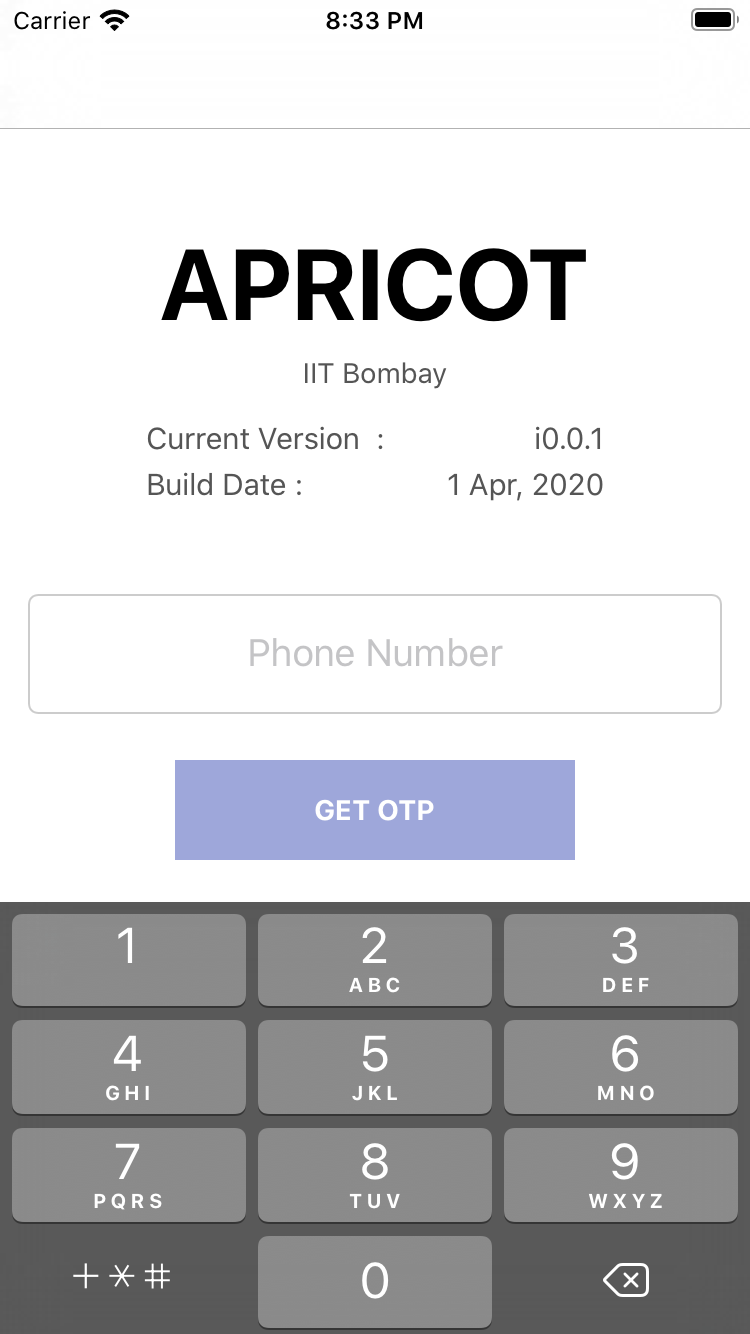
\includegraphics[width=.5\linewidth]{login1.png}
    \caption{Phone Number Input}
    \label{fig:sub1}
  \end{subfigure}%
  \begin{subfigure}{.5\textwidth}
    \centering
    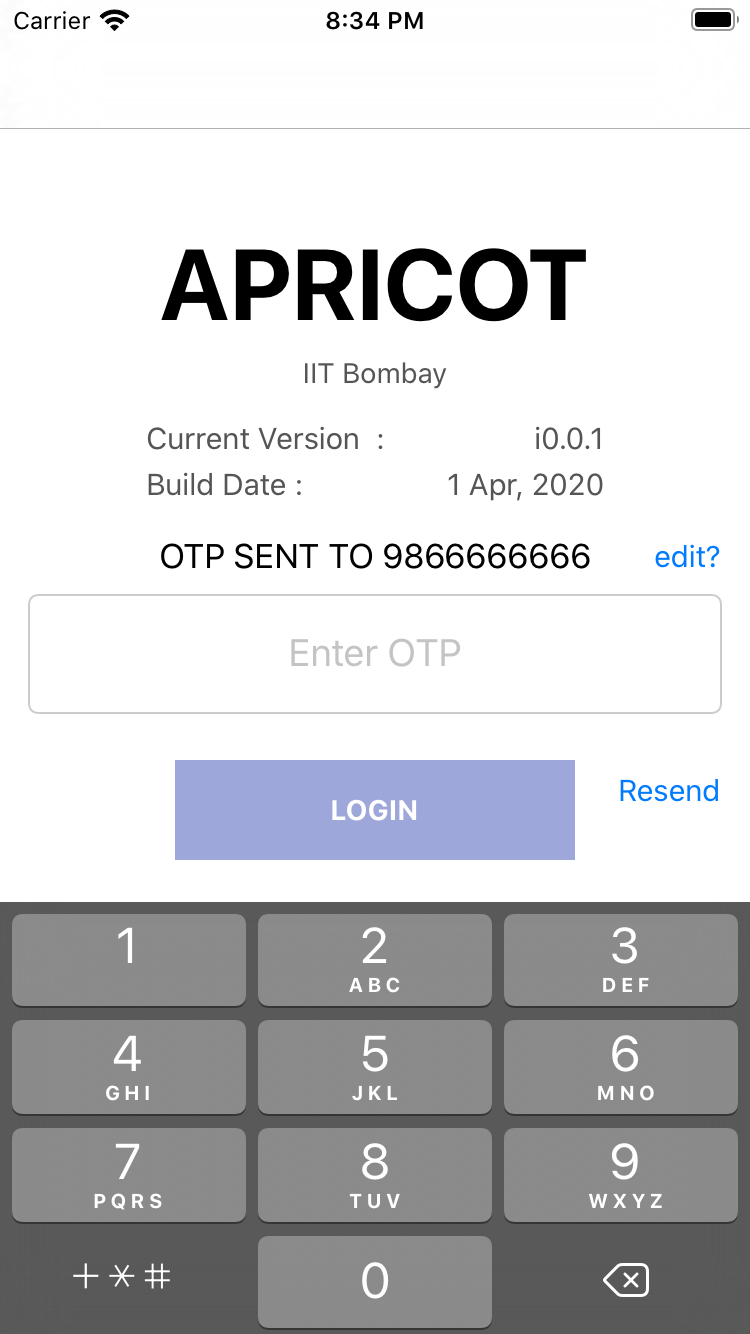
\includegraphics[width=.5\linewidth]{login2.png}
    \caption{OTP Input}
    \label{fig:sub2}
  \end{subfigure}
  \caption{The login Screen}
  \label{fig:login}
  \end{figure}
\newpage
The input field takes numbers up to 10 digits. Restricting the phone number field to 10 digits is done using the \mintinline{swift}{phoneNumFieldDidChange} function. The function is set to be triggered whenever the input field changes using the following lines of code:
\begin{minted}{swift}
  phoneNumberInput.addTarget(self, 
                             action: #selector(phoneNumFieldDidChange), 
                             for: UIControl.Event.editingChanged)
\end{minted}
The \mintinline{swift}{phoneNumFieldDidChange} function is as follows: 
\begin{minted}{swift}
  @objc func phoneNumFieldDidChange(){
      var phoneNumberCount = 0
      if let phoneNumber = phoneNumberInput.text {
          phoneNumberCount = phoneNumber.count
      }
      if(phoneNumberCount < 10) {
          getOTPButton.isEnabled = false
          getOTPButton.alpha = 0.5
      }else {
          if(phoneNumberCount > 10) {
              phoneNumberInput.deleteBackward()
          }
          getOTPButton.isEnabled = true
          getOTPButton.alpha = 1
      }
  }
\end{minted}
On touching the \textbf{GET OTP} button the function \mintinline{swift}{getOTP()} is called. The \mintinline{swift}{getOTP()} function stores the entered phone number in the \mintinline{swift}{GlobalFn} class and then calls the \mintinline{swift}{apiToGenerateOTP} function. 
\begin{minted}{swift}
  @objc func getOTP(){
      let phoneNumber = phoneNumberInput.text!
          GlobalFN().phoneNum =  phoneNumber
          apiToGenerateOTP()
      }
\end{minted}
The \mintinline{swift}{apiToGenerateOTP} function first shows a loading indicator using \textcolor{pink}{SwiftSpinner} class. 
\begin{minted}{swift}
 SwiftSpinner.show("Sending OTP")  
\end{minted}
Then it prepares the parameters for the API call. The required parameters are:
\begin{itemize}
  \item \textbf{\mintinline{swift}{phone:}} Phone number entered by the user to which the OTP is to be sent
  \item \textbf{\mintinline{swift}{device_id:}} This is a unique ID used to identify this particular device at the server. 
  \item \textbf{\mintinline{swift}{app_id:}} This is a unique ID used by the backend to identify a particular app version and on the OS which it is running.
\end{itemize}

\textbf{Generating unique device ID in iOS\\}\\
Early iOS releases provided a unique identifier for each device. But then this identifier was used by developers to uniquely identify a particular user. This was a security concern for Apple. Hence they changed the unique identifier with a vendor-specific device identifier. The identifier’s value is the same for apps from the same vendor on the same device. But it’s different for other vendors on the same device. The unique identifier is provided from the App Store. If the app is not present on the App Store then the identifier is derived from the bundle identifier of the App. 
Here is how to get the unique identifier. 
\begin{minted}{swift}
 let uuid = UIDevice.current.identifierForVendor?.uuidString   
\end{minted}
The UUID is going to be the same for every launch of the App. However, if the user uninstalls the app and re-installs it then the UUID will change. To keep the UUID the same even after re-install we should save the UUID in the keychain. The entries in keychain are kept even after the app is uninstalled unless the user clears them explicitly. The UUID is stored in a property named \mintinline{swift}{keychainUniqueDeviceId} in the \mintinline{swift}{GlobalFn} class. When the app starts for the first time this value is an empty string. In the \mintinline{swift}{AppDelegate} class, this value is checked and if it’s an empty string then the value is generated and saved in the keychain as follows: 
\begin{minted}{swift}
  if(GlobalFN().keychainUniqueDeviceId == ""){
      if let uuid = UIDevice.current.identifierForVendor?.uuidString{
          GlobalFN().keychainUniqueDeviceId = uuid;
      }
   }
\end{minted}
Afterward, the \mintinline{swift}{keychainUniqueDeviceId} is accessed from the \mintinline{swift}{GlobalFn} class. The getter and setter are defined as follows:
\newpage
\begin{minted}{swift}
    var keychainUniqueDeviceId:String {
            get {
                let bundleName = Bundle.main.bundleIdentifier
                let keychain = Keychain(service: bundleName ?? "apricot")
                if let id = keychain[UniqueDeviceKey]  {
                    return id
                }
                return ""
            }
            set {
                let bundleName = Bundle.main.bundleIdentifier
                let keychain = Keychain(service: bundleName ?? "apricot")
  
                if let t = keychain[UniqueDeviceKey]  {
                    print("key already saved : "+t)
                }
                else {
                    keychain[UniqueDeviceKey] = newValue
  
                }
                
            }
        }
\end{minted}
\textbf{The \mintinline{swift}{app_id:}}\\
The \mintinline{swift}{app_id} is set as required by the back-end. It’s a string used to identify a particular version of the app. 
After constructing the parameter dictionary as follows:
\begin{minted}{swift}
  let parameters : [String : String] = [
            "phone" : GlobalFN().phoneNum as String,
            "device_id" :    GlobalFN().keychainUniqueDeviceId,
            "app_id" : GlobalFN().app_id
        ]
\end{minted}
The dictionary is converted to JSON and then the appropriate format required by the API using,
\begin{minted}{swift}
  let jsonString = GlobalFN().dictToJSON(dict: parameters as NSDictionary)
  let jsonData = jsonString.data(using: .utf8)!
  let attListRequest = 
              try! JSONDecoder().decode(otpRequest.self, from: jsonData)
\end{minted}
And finally, we make the API call using,
\begin{minted}{swift}
  ApricotAPIManager.generateOTP(lastUpdateRQ:attListRequest)
\end{minted}
The API end-point for generating OTP is:
\begin{minted}{swift}
	BASE_URL+"api/v1/login/generate-otp/"
\end{minted}
This value of the \mintinline{swift}{BASE_URL} as picked up from the  \mintinline{swift}{ApricotNetworkURL.plist}  file.
The callback function is written as a closure. The function is called when the API returns either success or error. If the API returns success then we load the OTP screen by calling the function:
\begin{minted}{swift}
	self.waitForOTP()
\end{minted}

The \mintinline{swift}{self} keyword is important because we are calling the function from a closure.\\\\
The \mintinline{swift}{waitForOTP} function does the following:
\begin{itemize}
  \item Updates the \mintinline{swift}{OTP SENT TO} text with the user’s phone number and also makes it visible. 
  \item Makes the \mintinline{swift}{editPhoneNumButton} and \mintinline{swift}{Resend OTP} button visible. 
  \item Disables the \mintinline{swift}{Resend OTP button} and sets a timer to enable it after \mintinline{swift}{OTP_MIN_INTERVAL} seconds, stored in \mintinline{swift}{GlobalFn} class. The timer is stored in the property \mintinline{swift}{otpTimer}. It will be used to re-start or invalidate the timer. 
  \item Changes the \mintinline{swift}{GET OTP} button label to \mintinline{swift}{LOGIN} and changes the function it triggers to \mintinline{swift}{checkOTPAndLogin} 
  \item Changes the placeholder of the input field to \mintinline{swift}{Enter OTP}
  \item Changes the listener function for the phone number input to \mintinline{swift}{OTPInputDidChange}
  \item Hides the SwiftSpinner popup. 
\end{itemize}
After which the screen looks as shown in figure \ref{fig:sub2}\\
The input field used for the phone number is used for OTP too. The function \mintinline{swift}{OTPInputDidChange} checks for the entered OTP and enables the \mintinline{swift}{LOGIN} button when the OTP length reaches the \mintinline{swift}{OTP_LENGTH} defined in \mintinline{swift}{GlobalFn} class. Currently, this value is 6. This function is very similar to the phone number equivalent function but kept them different to improve readability.\\ 
After \mintinline{swift}{OTP_MIN_INTERVAL} the user can click on the \mintinline{swift}{Resend?} button and regenerate the OTP. The API used for generating the OTP is used for re-generating too. 
The user can click on the \mintinline{swift}{edit?} button to edit the phone number and resend the OTP. The \mintinline{swift}{loadPhoneNumber} function manages this. 
Once the user enters the six-digit OTP and clicks on \mintinline{swift}{LOGIN} the\mintinline{swift}{verify-otp} API is called from the function \mintinline{swift}{apiToVerifyOTP}. The API call is similar to \mintinline{swift}{generate-otp} and has only one extra parameter, the OTP entered by the user. 
The API end-point is:
\begin{minted}{swift}
	"api/v1/login/verify-otp/"
\end{minted}
If the OTP is correct the API returns a success message and the following: 
\begin{itemize}
  \item \textbf{\mintinline{swift}{token}}: A unique login token to determine if the user is logged in. 
  \item \textbf{\mintinline{swift}{user_id}}: A unique ID maintained at the back-end.
  \item \textbf{\mintinline{swift}{pseudo_id_list}}: A list of pseudo ID’s to be used for Bluetooth scanning and broadcasting.
\end{itemize}
After receiving these, the values are stored in the User Defaults which is a persistent key-value storage for iOS apps to store small values. The getters and setters for these values are defined in the \mintinline{swift}{GlobalFn} class. 
\newpage
Saving the values: 
\begin{minted}{swift}
  GlobalFN().token = valueDict["token"] as! String
  GlobalFN().user_id = valueDict["user_id"] as! String
  GlobalFN().pseudo_id_list = valueDict["pseudo_id_list"] as! NSArray
\end{minted}
Getters and Setters: 
\begin{minted}[fontsize=\footnotesize]{swift}
 var token: String {
    get {
        if let returnValue = UserDefaults.standard.object(forKey: "token") as? String {
            return returnValue
        } else {
            return "" //Default value
        }
    }
    set {
        UserDefaults.standard.set(newValue, forKey: "token")
        UserDefaults.standard.synchronize()
    }
  }
\end{minted}
Storing the \mintinline{swift}{user_id} is similar. The \mintinline{swift}{pseudo_id_list} is an array of 1000 pseudo ID's. The device chooses one of them to broadcast, and it changes the ID every 5 minutes. This enables the privacy of the user. 
The array is stored in UserDefaults. So that once logged in, the array is directly read from the local storage without needing an API call. 
Since the pseudo ID list is an array, to retrieve it, we need to cast it as an \mintinline{swift}{NSArray}. 
\begin{figure}[!htbp]
  \centering
  \begin{subfigure}{.5\textwidth}
    \centering
    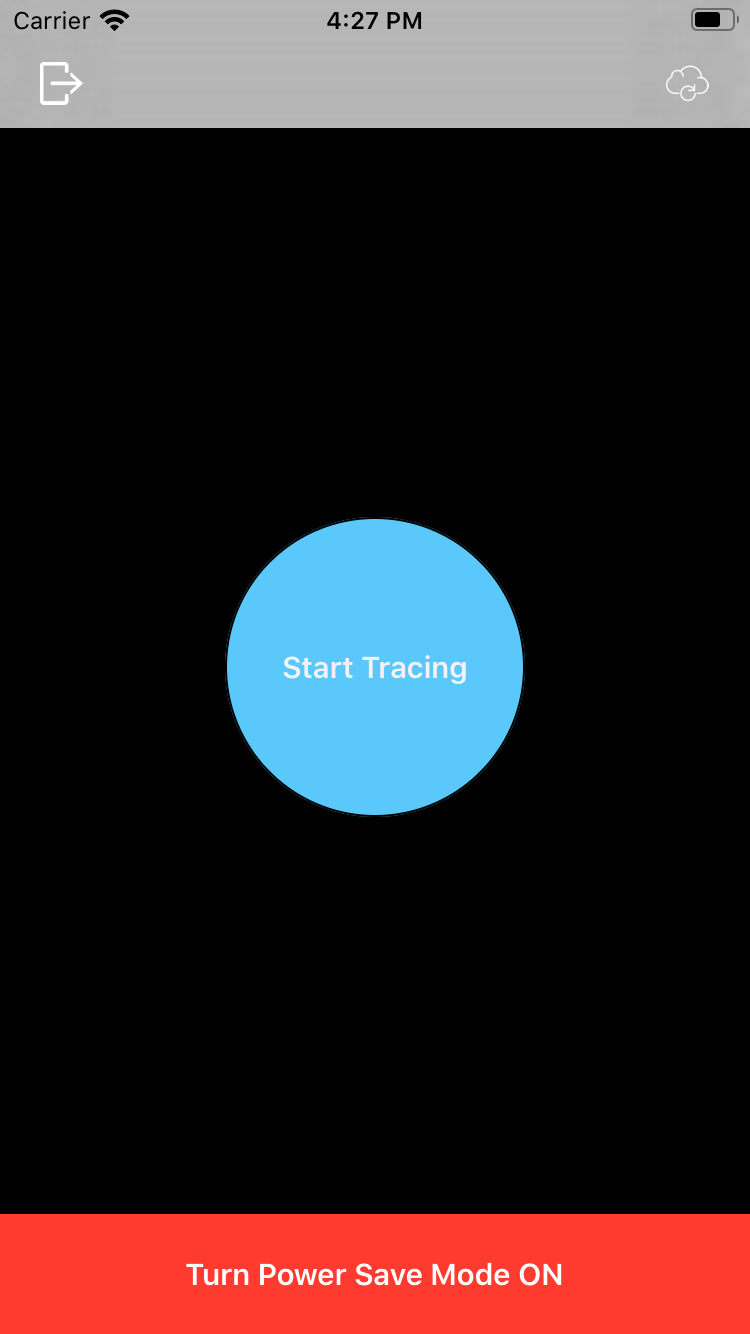
\includegraphics[width=.5\linewidth]{trace1.png}
    \caption{Tracing off}
  \end{subfigure}%
  \begin{subfigure}{.5\textwidth}
    \centering
    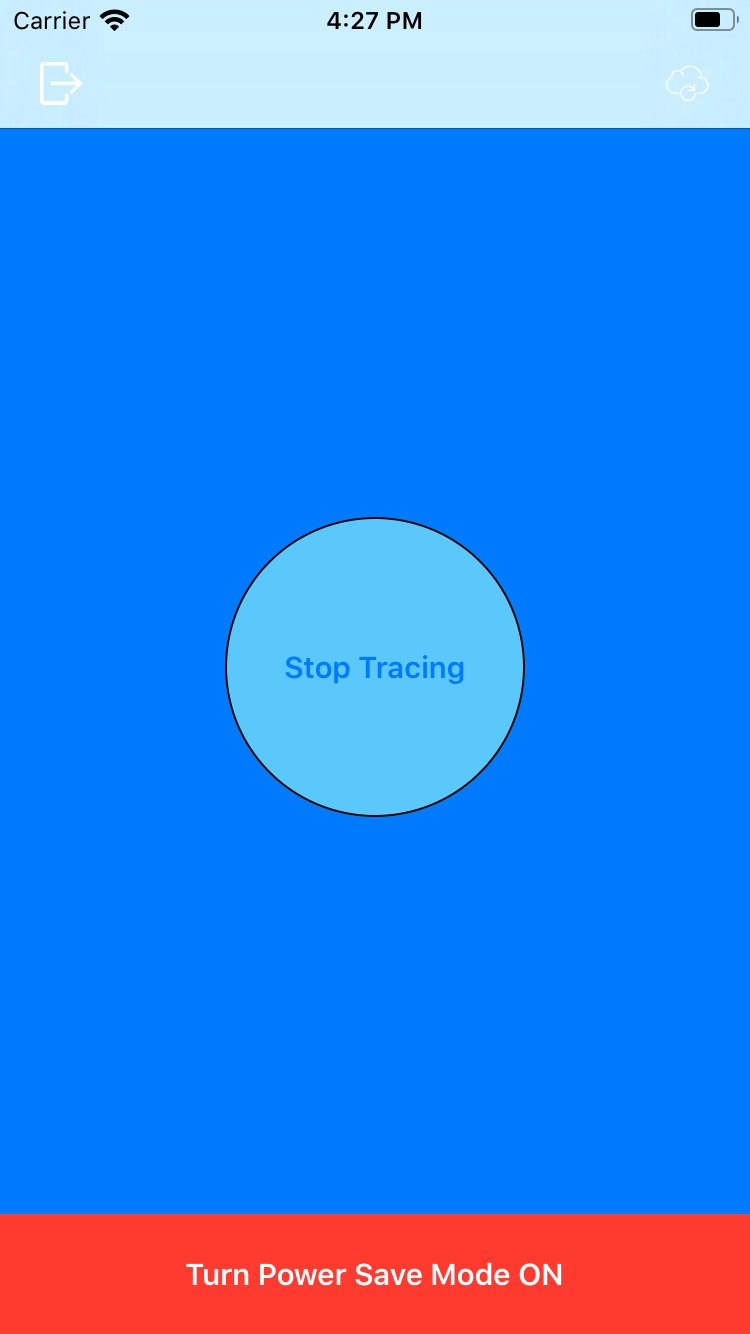
\includegraphics[width=.5\linewidth]{trace2.png}
    \caption{Tracing on}
  \end{subfigure}
  \caption{The Main Screen}
  \label{fig: trace}
\end{figure}
\newpage
Once the user is logged-in, the main Bluetooth scanning screen is loaded with animation using:
\begin{minted}[fontsize = \footnotesize]{swift}
 let storyboard = UIStoryboard(name: "Trace", bundle: nil)
 let vc = 
  storyboard.instantiateViewController(withIdentifier: "TraceVC") as! TraceViewController
 self.pushViewControllerWithTransition(vc: vc)
\end{minted}

The \mintinline{swift}{pushViewControllerWithTransition} function pushes the \mintinline{swift}{TraceVC}  view controller on top of the screen with a \mintinline{swift}{flip} animation. The user then sees the screen in figure \ref{fig: trace}

On clicking\mintinline{swift}{Start Tracing}. The app begins scanning for Bluetooth devices broadcasting their pseudo ID's nearby. It also broadcasts its own pseudo ID. 
The app then stores the pseudo ID of nearby devices with timestamp locally. Each phone scans for the nearby devices for a time of 1 min. The contact trace history is deleted after 30 days.
Using the upload button, the user can upload his contact trace to the server. 
iOS uses iBeacon for Bluetooth beaconing. There is one challenge in iOS. We have a limited number of bits for pseudo ID (16 bits). This restriction is not present in Android.
In the future, we plan to use Eddy Beacon and iBeacon both to increase this limit. 
Currently, if the user exits from the app, the app stops scanning. Hence we encourage users to keep the app in the foreground. That is why we provide a power-saving mode which 
reduces the brightness to zero. 


\section{Acknowledgement}
\label{SEC:acknowledgement}
I thank Prof. Bhaskaran Raman for giving me the opportunity to work on these interesting projects and also for his valuable guidance during the process. 

\newpage
\nocite{*}
\printbibliography
\end{document}          
